\chapter{Introduction}\label{chap:intro}
\section{The Conception of Semiconductors}\label{sec:semicond_conception}
Here we present work by \cite{Mott_PhysRev1969, Allen_Nature1960}.

\begin{table}[h]
	\centering
	\begin{threeparttable}
	\begin{tabular}{c c c c c}
		\hline\hline
		Semiconductor & \multicolumn{1}{p{3cm}}{\centering Band Gap \\($\mathrm{eV}$)} & \multicolumn{1}{p{3cm}}{\centering Electron Mobility\tnote{1} \\ ($\mathrm{cm}^2/\mathrm{V}\cdot\mathrm{s}$)} & \multicolumn{1}{p{3cm}}{\centering Hole Mobility\tnote{1} \\ ($\mathrm{cm}^2/\mathrm{V}\cdot\mathrm{s}$)} & \multicolumn{1}{p{3cm}}{\centering Lattice Constant \\ (\r{A})} \\ [0.5ex]
		\hline
		\ch{Si} & 1.12 & 1,500 & 470 & 5.43095\tnote{a}\\
		\ch{Ge} & 0.67 & 3,900 & 1,900 & 5.64613\tnote{a}\\ 
		\ch{GaAs} & 1.42 & 8,500 & 400 & 5.6533\tnote{b}\\
		\ch{CdS} & 2.5 & 300 & 50 & 5.8320\tnote{c}\\
		\ch{AlAs} & 2.16 & 1,200 & 400 & 5.6622\tnote{b}\\
		\ch{ZnS} & 3.66 & 165 & 5 & 5.410\tnote{d}\\[1ex]
		\hline
		\label{table:semiconductor_props}
	\end{tabular}
	\caption[Properties of selected semiconductors]{Selected properties of some common semiconductors at $T=300\,\mathrm{K}$. Adapted from ref.~\cite{Schroder_Semiconductor2006}.}
	\begin{tablenotes}
		\item[1] Drift mobilities in the purest materials.
		\item[a] Diamond cubic crystal structure \cite{Omara_Handbook1990}.
		\item[b] Zinc blende crystal structure \cite{Moss_Semiconductor1989}.
		\item[c] Hexagonal and cubic... citation needed.
		\item[d] Notes on \ch{ZnS} structure.
	\end{tablenotes}
	\end{threeparttable}
\end{table}

\begin{figure}[ht]
	\centering
	\begin{minipage}[b]{0.45\linewidth}
		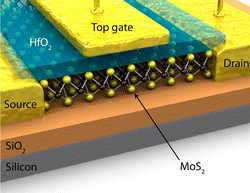
\includegraphics[height=3cm,width=5cm]{figs/mos2fet}
		\caption{Name}
		\label{fig:minipage1}
	\end{minipage}
	\qquad
	\begin{minipage}[b]{0.45\linewidth}
		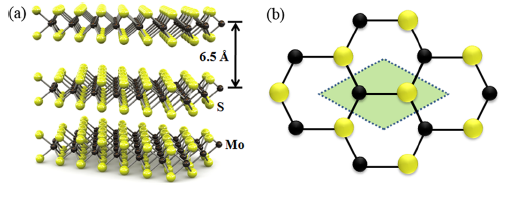
\includegraphics[height=3cm,width=5cm]{figs/mos2diagram}
		\caption{name}
		\label{fig:minipage2}
	\end{minipage}
\end{figure}

\begin{figure}[ht]
	\centering
	\subfigure[Short caption]{
	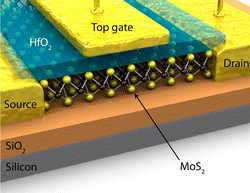
\includegraphics[height=2cm,width=3cm]{figs/mos2fet}
	\label{fig:subfig1}
	}
	\qquad
	\subfigure[sub fig2]{
	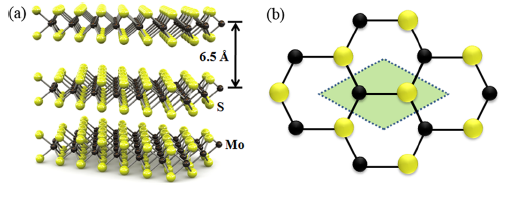
\includegraphics[height=2cm,width=3cm]{figs/mos2diagram}
	\label{fig:subfig2}
	}

	\subfigure[sub fig3]{
	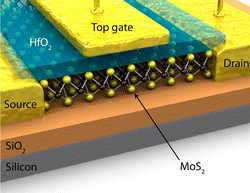
\includegraphics[height=2cm,width=3cm]{figs/mos2fet}
	\label{fig:subfig3}
	}
	\qquad
	\subfigure[sub fig4]{
	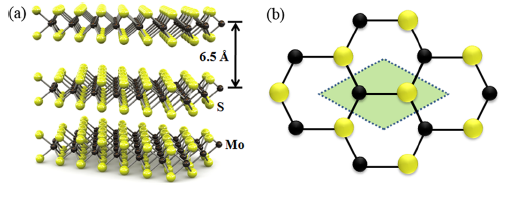
\includegraphics[height=2cm,width=3cm]{figs/mos2diagram}
	\label{fig:subfig4}
	}
	\caption{main caption}
	\label{fig:figure}
\end{figure}

\section{Evolution of Semiconductors}\label{sec:semicond_evolution}

\section{Interest and Development of Two-dimensional Materials}\label{sec:2D_development}

\section{Current State of Two-dimensional Materials}\label{sec:current_state}